%!TEX root = main.tex

\subsection{What is NLP ?}

Natural language processing (NLP) is a field of computer science, artificial intelligence, and computational linguistics concerned with the interactions between computers and human (natural) languages. There is differents applications:
\begin{itemize}
	\item Communicating agent;
	\item Translator;
	\item Information extraction;
	\item Inference of knowlegde;
	\item \dots
\end{itemize}

\subsection{Three approches to NLP}

\begin{enumerate}
	\item \textbf{Symbolic}: Use of language ressources (dictionnaries, grammars, thesaurus, \dots);
	\item \textbf{Statistical}:  Use of empirical techniques to learn from text and construct language models;
	\item \textbf{Hybrid}: Combining language ressources and statistical algorithms.
\end{enumerate}

\subsection{Basic linguistics concepts}

\subsubsection{Language vs. languages}

\begin{itemize}
	\item \textbf{A language}: A system of spoken/written communication used by a particular country, people, \dots typically consisting of words used within a regular grammatical and syntactic structure;
	\item \textbf{The language}: Power or faculty of speech.
\end{itemize}


\subsubsection{Competence vs. performance}

\begin{itemize}
	\item \textbf{Competence}: knowledge of a language;
	\item \textbf{Performance}: Use of language in concrete situation.
\end{itemize}

\subsubsection{Nature of the linguistic sign}

\textit{Words} are \textit{linguistic signs}. They convey some idea.

\noindent
\begin{minipage}{.5\textwidth}
	\begin{itemize}
		\item \textbf{Signifier}: The psychic imprint of the sound (not the sound);
		\item \textbf{Signified}: The concept associated to the signifier;
		\item \textbf{Referent}: Actual \textit{object} in the real world.
	\end{itemize}
\end{minipage}%
\begin{minipage}{.5\textwidth}
	\centering
	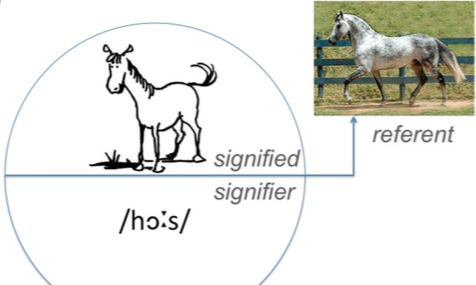
\includegraphics[scale=0.4]{images/01_nature.png}
 	\captionof{figure}{Nature of linguistic sign.}
\end{minipage}

\vspace{10px}

The linguistic sign has the three following characteritics:

\begin{itemize}
	\item \textbf{Arbitrary}: The relationship between the signifier and the signified is not motivated;
	\item \textbf{Conventional}: The link is based on social conventions;
	\item \textbf{Differential}: Signs are part of a system.
\end{itemize}


\subsubsection{Double articulation of the language}

A double articulation caracterize human languages.

\begin{itemize}
	\item At first level, \textbf{morpheme} (or moneme) are the smallest meaningful units. A \textbf{morph} is a concrete realisation of a morpheme. For example, the morphene \textit{take} has two realizations: \textit{take, took}. The variants of a same morpheme are called \textbf{allomorphs};
	\item At a second level, \textbf{phonemes} are the smallest distinctive units. A \textbf{phone} is a realisation of a phoneme. Variants of a given phoneme are called \textbf{allophone} (livre and ville).
\end{itemize}

\subsubsection{Two axes: syntagmatic vs. paradigmatic}

\noindent
\begin{minipage}{.4\textwidth}
	Morphemes can be replaced by others on the \textbf{paradigmatic} axis (vertical) or they can appear in a different environement, combined with other morphemes on the \textbf{syntagmatic} axis (horizontal).
\end{minipage}%
\begin{minipage}{.6\textwidth}
	\centering
	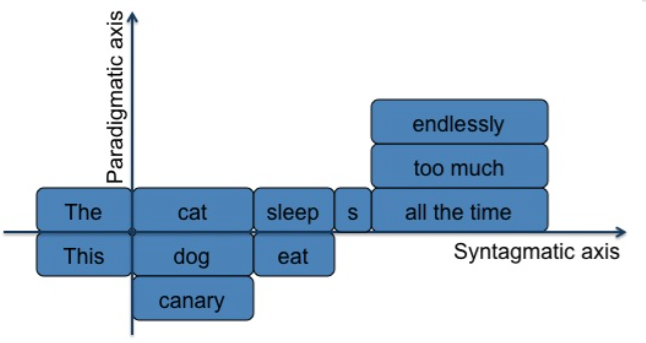
\includegraphics[scale=0.4]{images/02_axis.png}
 	\captionof{figure}{The two axes.}
\end{minipage}

\subsubsection{Other general linguistic considerations}

\begin{itemize}
	\item \textbf{Creativity}: Finite number of signs permit to elaborate an infinite number of utterences;
	\item \textbf{Evolutivity}: Languages change over the time;
	\item \textbf{Complexity}: Languages are of equal complexity.
\end{itemize}

\subsection{Levels of a linguistic analysis}

\begin{figure}[htp]
	\centering
	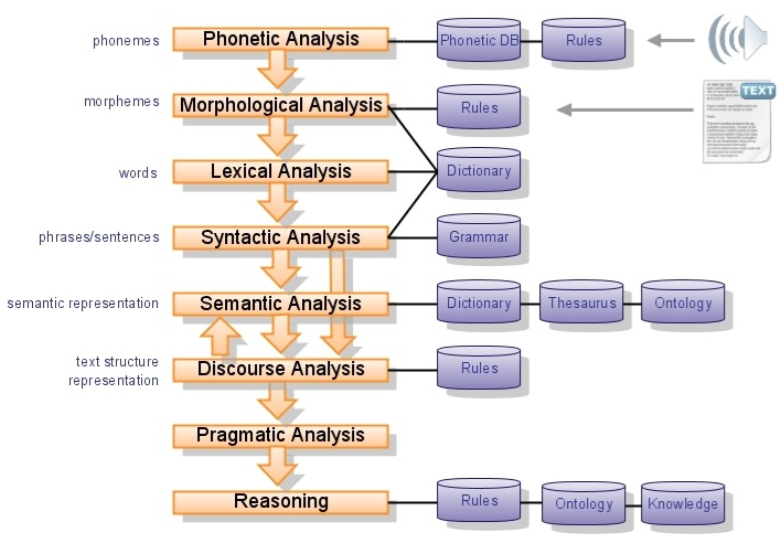
\includegraphics[scale=0.4]{images/03_levels.png}
 	\caption{Different levels of linguistic analysis.}
\end{figure}

\subsubsection{Phonology}

It is the systematic study of the sounds used in language, and their composition into syllables, words, phrases. Computational phonology is the application of formal and computational techniques to the representation and processing of phonological information.

\vspace{10px}
There is several applications:
\begin{itemize}
	\item Speech recognition;
	\item Speech synthesis;
	\item Phonetic algorithms;
	\item \dots
\end{itemize}

\subsubsection{Morphology}

The notion of word is ambiguous:
\begin{itemize}
	\item \textbf{Tokens}: Number of words; \textbf{Types}: Number of unique words.
	\item \textbf{Phonemic} words: \textit{[hai]}; \textbf{Graphemic} words: \textit{high}.
	\item \textbf{Mono-lexical} unit: \textit{feuille}; \textbf{Polylexical} unit: \textit{arc-en-ciel}.
	\item \textbf{Function} word: \textit{to, from}; \textbf{Full} word: \textit{home, sea}.
\end{itemize}

\vspace{10px}

There is too abstract notions behind words:
\begin{itemize}
	\item \textbf{Lemma}: Is the cannonical form of a word (entry of a dictionary, infinitive form or masculine form);
	\item \textbf{Part of Speech}: Are grammatical categories indentifying the nature and/or syntactic function of a word.
\end{itemize}

\vspace{10px}

Morphene are abstract entities expressing semantic concepts or grammatical features.

\begin{figure}[htp]
	\centering
	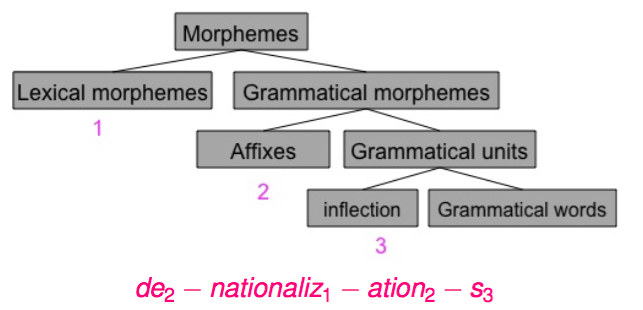
\includegraphics[scale=0.4]{images/04_tree.png}
 	\caption{Grammatical and Lexical morphology.}
\end{figure}

There is several ways to create new words:

\begin{itemize}
	\item \textbf{Inflection}: Grammatical adaptation of a word in a particular syntactic contexts (grammatical morphology);
	\item \textbf{Derivation}: Creation of a new word by adding a bound morpheme (affix) to a derivational base (lexical morphology);
	\item \textbf{Composition}: joining of two or more base forms: hot pepper, cool-headed, online, \dots
\end{itemize}

\vspace{10px}


There are three main aspects linked to morphological analysis:

\begin{itemize}
	\item \textbf{Lemmatization \& Stemming}: The goal is to reduce inflectional forms and sometimes derivationally related forms of a word to a common base form.
	\begin{itemize}
		\item \textbf{Lemmatization}: Based on morphological dictionnaries and analyzers. \textbf{Morphological analyser}  are able to analyze new words using a base dictionary (words and affixes) and morphological rules (add/remove affixes). \textbf{Morphological dictionaries} contain forms, lemma, morphological information, \dots.
		\item \textbf{Stemming}: Based on predefined rules.\\
		Algorithm of Porter: 
		\begin{enumerate}
			\item Check if word respect some form;
			\begin{figure}[htp]
				\centering
				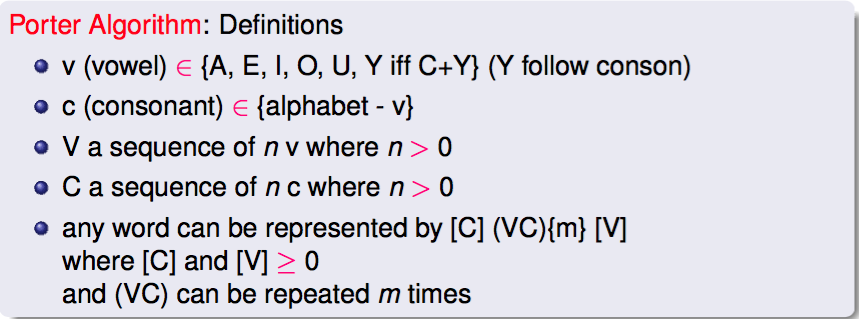
\includegraphics[scale=0.4]{images/05_form.png}
			\end{figure}
			\item If word respect some form, apply 5 runs of somes rules.
			\begin{figure}[htp]
				\centering
				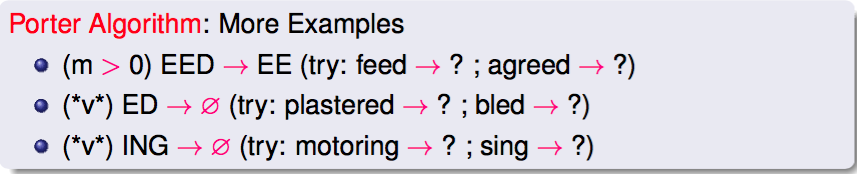
\includegraphics[scale=0.4]{images/06_rule.png}
			\end{figure}
		\end{enumerate}
		There is two typical problems: \textbf{Under-stemming} error (algo failed to group two words sharing conceptual meaning: divide and division does not give the same result); \textbf{Over-stemming} error (algo grouped words having no shared conceptual meaning: wand and to wander).
	\end{itemize}
	\item \textbf{POS Tagging}: labeling word with POS (rules vs probabilities);
	\item \textbf{Disambiguation}: Clarify the nature or function of a word in a sentence.
\end{itemize}


\subsubsection{From lexis to syntax}

Lexicalization is the process of adding words, set phrases, or word patterns to a language. This step is complicated for \textbf{compound words} and \textbf{frozen expressions}.